\documentclass[aspectratio=169]{beamer}
\usetheme{metropolis}
% \usetheme{gotham}
% \useoutertheme[
%   progressbar position=foot,   % 进度条位置:foot/head/none
%   progressbar style=rectangle, % 样式:rectangle/rounded box/circle
%   numbering=totalframenumber   % 页码样式:none/framenumber/totalframenumber
% ]{gotham}

\usefonttheme{professionalfonts} % 使用系统/自定字体


% === 字体设置 ===
\usepackage[UTF8,scheme=plain,fontset=none]{ctex}
\setCJKmainfont{Source Han Serif CN}[BoldFont={Source Han Serif CN Bold}]
\setCJKsansfont{Source Han Sans CN}[BoldFont={Source Han Sans CN Bold}]
% \setCJKmonofont{Sarasa Mono CN}


% beamer 已加载 hyperref;加 unicode 以支持中文书签
\hypersetup{unicode}

% define paragraph
\providecommand{\paragraph}[1]{\smallskip\textbf{#1}\par}

% 常用包
\usepackage{longtable,booktabs}
\usepackage{amsmath,amssymb}
\usepackage{graphicx}
\graphicspath{{.}{./figs/}{./images/}{./images_in_paper/}}
\usepackage{caption}
\usepackage{subcaption}
\usepackage{float}
\usepackage{svg}
\usepackage{booktabs}
\usepackage{array}
\usepackage{threeparttable}

% 超链接(beamer 已加载 hyperref,这里只补选项)
% \hypersetup{unicode=true}

% 编号风格
\setbeamertemplate{caption}[numbered]
\setbeamertemplate{caption label separator}{.}

\title{从时域到频域:基于多分支CNN网络的AI音频检测模型}
\author{NKUMMF2025138}
\date{\today}


%---Document Begins---
\begin{document}

\begin{frame}
  \titlepage
\end{frame}


% 摘要页(无页眉,允许自动换页)
\begin{frame}[plain,allowframebreaks]{摘要}
\small

% \begin{center}
%   \textbf{\huge 摘\quad 要}
% \end{center}
\vspace{0.2cm}

\begin{abstract}
针对AI音频的识别问题,本文提出一种基于\textbf{多分支卷积神经网络(Multi-Branch CNN)}的
端到端 AI 音频检测与评分模型。

从\textbf{时域、频域及声学常见统计量}等多角度提取 11 类特征,分别经五个并行分支建模后融合判别。
针对单分支贡献的量化问题,引入\textbf{分支探针}机制,
基于各分支独立判别准确率确定加权系数,构建可解释的 AI 痕迹综合评分体系。

本文设计多种扰动与对抗性处理(如频谱均衡、高频注入、环境噪声混入等)评估模型鲁棒性,并结合分支贡献分析揭示其在时域包络与共振峰布局上的依赖性。实验结果表明,该模型在验证集上准确率可达 89\%–90\%,在多数轻中度扰动下保持稳定性能,综合评分在强扰动下亦具较高稳健性。本文方法具有较低计算开销与良好可扩展性,可推广至语音伪造检测、环境音识别等领域。

\end{abstract}

\vspace{0.5em}
\noindent\textbf{关键词:} AI 音乐检测;多分支CNN;音频特征提取;探针机制;AI 痕迹评分

\end{frame}




\section{判别模型的建立与求解}

\begin{frame}[fragile,allowframebreaks]{模型建立与求解}
\small
\begin{enumerate}
  \item{模型假设}
  \item{数据处理}
  \item{特征说明}
  \item{模型建立}
  \item{结果分析}
\end{enumerate}
\end{frame}

\subsection{模型假设}
\begin{frame}[fragile,allowframebreaks]{模型假设}
\small
\begin{enumerate}
    \item 人工标注的“真人/AI”标签总体正确率较高;
    \item 在选定的分析窗口($20$s)内,音频的统计特性近似平稳,从而帧级特征的统计聚合是有效的。
\end{enumerate}
\end{frame}

\subsection{数据处理}
\begin{frame}[fragile,allowframebreaks]{数据处理}
  \small
  \begin{enumerate}
    \item{代码中首先将输入文件转码为 WAV 格式}
    \item{采用音频处理领域常用的 $22050$ Hz 采样率对输入音频进行统一解码与重采样}
    \item{在特征提取流程中,原始歌曲首先被切分为 20 秒长度的片段}
  \end{enumerate}
在此基础上,本文提取了表~\ref{tab:audio-features} 中所列的多种时域、频域及声学特征,涵盖能量变化、频谱形状、谐波结构及共振峰等方面的信息。
\end{frame}

\subsection{特征说明}
\begin{frame}[fragile,allowframebreaks]{特征说明}
\begin{table}
  \centering
  \begin{tabular}{lll}
    \toprule
    特征名称 & 维度 & 特征类型 \\
    \midrule
    rms       & (1, 862)   & 时域能量 \\
    zcr       & (1, 862)   & 时域变化 \\
    hjorth    & (3, 1)     & 全局统计 \\
    log\_mel  & (128, 862) & 频域谱图 \\
    mfcc      & (13, 862)  & 声学特征 \\
    centroid  & (1, 862)   & 频谱形状 \\
    contrast  & (7, 862)   & 频谱对比度 \\
    flatness  & (1, 862)   & 频谱形状 \\
    f0        & (1440,)    & 音高曲线 \\
    hnr       & (1998,)    & 声学质量 \\
    formant   & (3, 2000)  & 共振峰 \\
    \bottomrule
  \end{tabular}
  \caption{各特征的名称、维度及类型}\label{tab:audio-features}
\end{table}
\end{frame}


\subsection{模型建立}
\begin{frame}[fragile,allowframebreaks]{模型建立}
本研究构建了一个多分支卷积神经网络(Multi-Branch CNN),用于融合处理多种类型的音频特征,从而实现对 AI 生成音频的准确识别。整体网络结构如下图所示,模型共由五个输入分支构成,分别对应不同特征类型,并通过特征融合实现最终的二分类判别。

\begin{figure}[h]
    \centering
    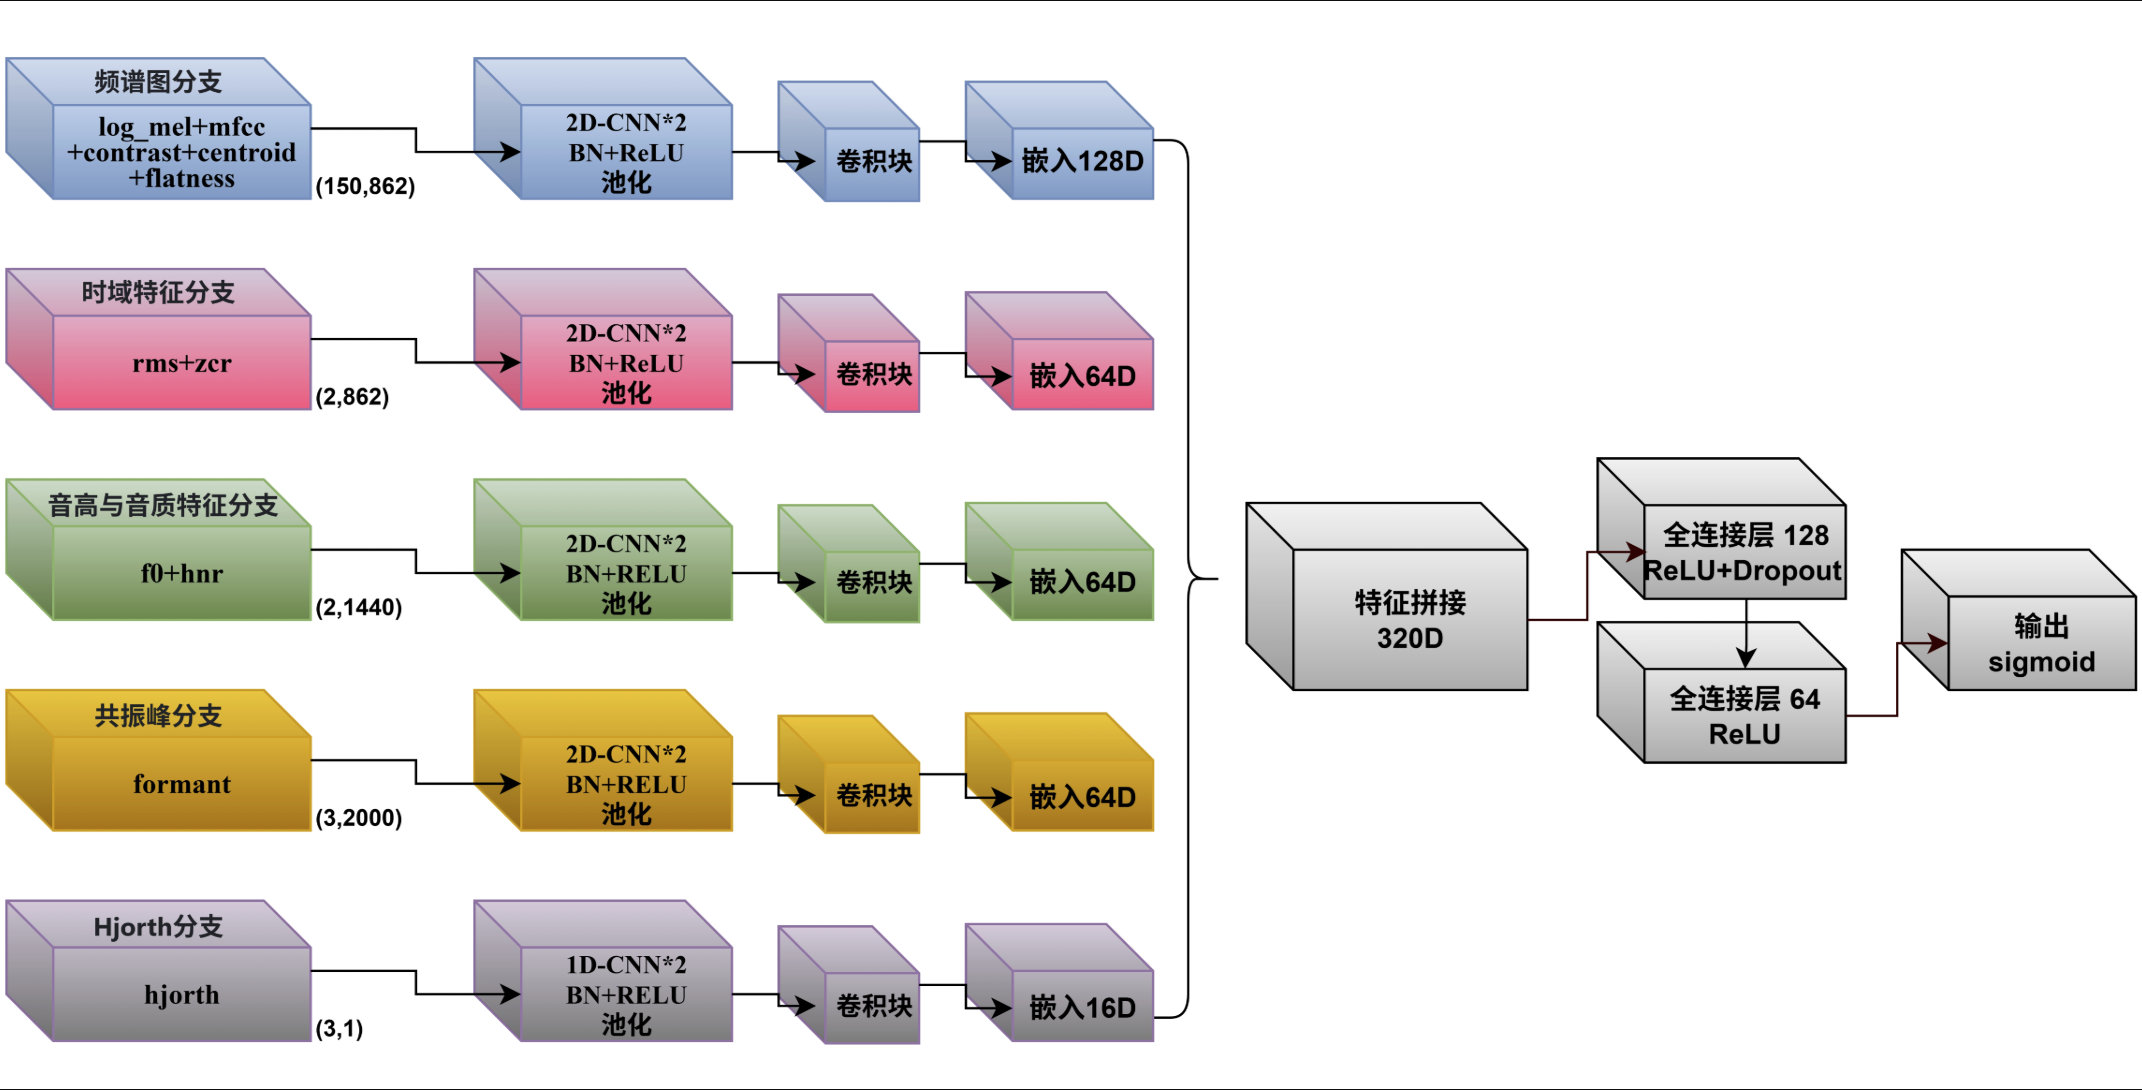
\includegraphics[width=0.75\linewidth]{images_in_paper/model.png}
    \caption{多分支CNN示意图}
    \label{fig:model}
\end{figure}

\end{frame}

\begin{frame}[fragile,allowframebreaks]{模型建立}

\begin{table}[h]
  \centering
  \small
  \resizebox{\textwidth}{!}{%
  \begin{tabular}{lll}
    \toprule
    \textbf{分支名称} & \textbf{输入特征} & \textbf{处理与输出} \\
    \midrule
    频谱图分支(Spectrogram) & log\_mel, mfcc, contrast, centroid, flatness & 2D CNN 提取时频模式 → GAP → 128 维表示 \\[2pt]
    时域分支(Time-Domain) & rms, zcr & 1D CNN 提取时间结构 → 64 维向量 \\[2pt]
    音高与音质分支(Pitch \& Quality) & f0, hnr & 1D CNN 建模调型与音质 → 64 维向量 \\[2pt]
    共振峰分支(Formant) & formant & 1D CNN 处理时间序列 → 64 维向量 \\[2pt]
    Hjorth 参数分支(Hjorth Param.) & hjorth (Activity, Mobility, Complexity) & 两层全连接 → 16 维表示 \\
    \bottomrule
  \end{tabular}%
  }
  \caption{多分支特征处理结构概览}
  \label{tab:branch-structure}
\end{table}

五个分支提取的特征向量分别为:128维(频谱图)、64维(时域)、64维(音高音质)、64维(formant)与16维(hjorth),合并后得到一个 $336$ 维的全局音频表征。该向量随后输入至全连接分类器,包含一层隐藏层(64单元),使用 ReLU 激活与 Dropout 防止过拟合,最终输出一个概率值,判定音频是否为 AI 生成。
\end{frame}


\subsection{结果分析}
\begin{frame}{结果分析}
\begin{figure}[htb]
  \centering
  \begin{subfigure}{0.48\linewidth}
    \centering
    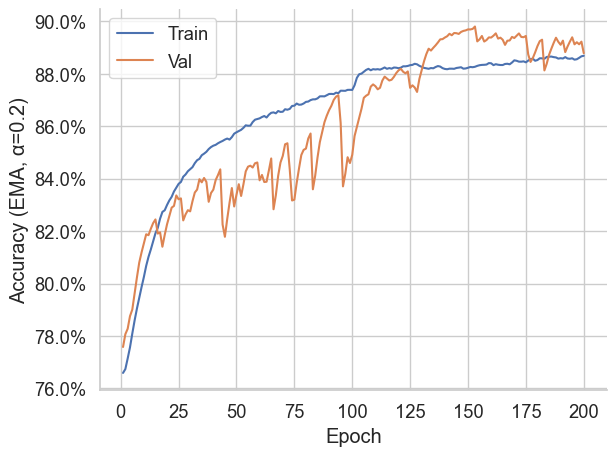
\includegraphics[width=\linewidth]{images_in_paper/acc_train_val.png}
    \caption{准确率(Train vs Val)}
    \label{fig:acc}
  \end{subfigure}\hfill
  \begin{subfigure}{0.48\linewidth}
    \centering
    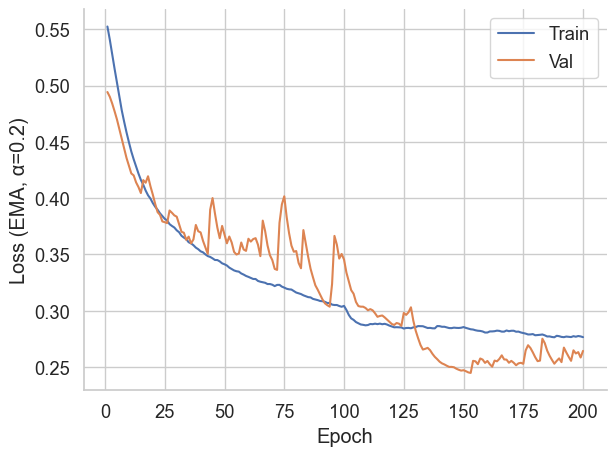
\includegraphics[width=\linewidth]{images_in_paper/loss_train_val.png}
    \caption{损失(Train vs Val)}
    \label{fig:loss}
  \end{subfigure}
  \caption{训练过程的准确率与损失对比}
  \label{fig:acc-loss}
\end{figure}
\end{frame}

\begin{frame}[fragile,allowframebreaks]{结果分析}

  训练损失呈单调递减趋势,最终趋近于0.27;

  训练集准确率从\textbf{76.5\%}持续上升并最终收敛于\textbf{88.5\%}左右,

  验证集准确率和损失虽经历多次波动,但最终趋于稳定,
  分别在\textbf{89\%-90\%}和\textbf{0.25-0.26}之间。
 
  上述结果表明模型训练稳定,未出现过拟合迹象。
  这说明多分支特征融合结构在提取不同维度音频信息时具有较好的\textbf{泛化能力},
  能够有效捕捉AI生成音乐与人类创作音乐的差异特征。

\end{frame}

\subsection{消融实验}
\begin{frame}[fragile,allowframebreaks]{消融实验}
为探究各输入分支在多分支 CNN 模型中的贡献度,本研究设计了消融实验,
通过控制不同分支的启用/关闭状态,评估其对模型分类精度的影响。
具体而言,我们分别在以下三种设置下进行测试:
\begin{itemize}
  \item 全分支开启;
  \item 单独关闭某一分支,其余保持开启;
  \item 单独开启某一分支,其余全部关闭。
\end{itemize}
\end{frame}

\begin{frame}[allowframebreaks]{消融实验}
\scriptsize
\begin{longtable}{cccccc}
\caption{消融实验结果(准确率 \%)\label{tab:ablation}}\\
\toprule
频谱图分支 & 时域分支 & 音高与音质分支 & 共振峰分支 & Hjorth 参数分支 & 准确率 \\
\midrule
\endfirsthead
\caption[]{消融实验结果(续)}\\
\toprule
频谱图分支 & 时域分支 & 音高与音质分支 & 共振峰分支 & Hjorth 参数分支 & 准确率 \\
\midrule
\endhead
\bottomrule
\multicolumn{6}{r}{\footnotesize 续下页…}\\
\endfoot
\bottomrule
\multicolumn{6}{l}{\footnotesize 注:1 表示该 CNN 分支传入真实特征张量,0 表示相同形状的全零张量。}\\
\endlastfoot
1 & 1 & 1 & 1 & 1 & 89.30\% \\
0 & 1 & 1 & 1 & 1 & 29.87\% \\
1 & 0 & 1 & 1 & 1 & 79.20\% \\
1 & 1 & 0 & 1 & 1 & 88.77\% \\
1 & 1 & 1 & 0 & 1 & 88.40\% \\
1 & 1 & 1 & 1 & 0 & 89.10\% \\
1 & 0 & 0 & 0 & 0 & 77.87\% \\
0 & 1 & 0 & 0 & 0 & 30.02\% \\
0 & 0 & 1 & 0 & 0 & 47.76\% \\
0 & 0 & 0 & 1 & 0 & 50.67\% \\
0 & 0 & 0 & 0 & 1 & 25.20\% \\
\end{longtable}

\end{frame}


\begin{frame}[fragile,allowframebreaks]{消融实验}
虽然消融实验能够衡量各分支在整体判别任务中的贡献度,但这种方法仍存在一定局限性:  
\begin{itemize}
  \item \textbf{无法独立量化单分支判别能力}:在消融实验中,关闭某一分支时其特征被替换为零向量,其余分支仍参与决策,因此所得精度下降值只是间接反映该分支的重要性,而非其独立完成任务的真实表现。  
  \item \textbf{分支间存在互补与冗余效应}:不同分支特征可能存在高度相关性,关闭一个分支后,其信息可能部分被其他分支补偿,导致重要性被低估;反之,如果多个分支特征冗余,关闭其中一个分支对结果影响可能被夸大。  
  \item \textbf{评估结果依赖当前模型权重分布}:消融实验是在固定训练好的多分支模型上进行的,权重分布已经针对多特征融合进行了优化,单分支输入下的表现可能不能代表该分支在独立训练时的潜力。  
  \item \textbf{未能刻画特征在不同类型样本上的贡献差异}:消融实验只给出整体平均精度,而没有分析分支在不同类别、不同难度样本上的表现差异,限制了对特征适用性的理解。  
\end{itemize}
针对以上不足,我们在后续模型中引入了分支探针机制,使每个分支能够在保持原有多分支协作的同时,单独完成二分类任务,从而获得更客观、细粒度的特征贡献评估结果。

\end{frame}



\section{评分机制}
\subsection{定义评分公式}
\begin{frame}{评分公式的定义}
受消融实验结果的启发,为了细化模型的评价指标,我们改进了多分支CNN网络,
为每个分支添加了一个由线性层和\texttt{Sigmoid}函数构成的\textbf{探针头结构}。

对于一段音频,每个分支的探针都可以独立判断该音频是否为AI生成,并输出\textbf{分类概率}。
\end{frame}

\begin{frame}[fragile,allowframebreaks]{评分规则}
% ========== 公式:评分规则 ==========
\paragraph{评分规则} 记各分支探针头给出的“音频为AI生成”的概率为
$p_i\in[0,1]$,则作品的综合评分(AI痕迹强度)定义为
\begin{equation}
    S \;=\; \sum_{i} \omega_i\, p_i \;\in\;[0,1],
    \label{eq:ai_score}
\end{equation}
其中 $\omega_i$ 为分支的评分权重。$S$ 越大表示该音频越可能为 AI 生成。
\end{frame}

\begin{frame}{分支权重的确定}
在综合各分支结果为音乐作品打分时,我们以各探针头单独决策时的\textbf{准确率}为依据,
确定了各分支的评分权重。

% ========== 公式:权重确定 ==========
设各分支探针在独立判别(AI/非AI)下的准确率
$acc_i,i\in\{\text{spec,time,prosody,formant,hjorth}\}$。

为避免随机猜测带来的偏置,先做机会校正(chance-corrected)并归一化:

\begin{equation}
    \omega_i \;=\; \frac{acc_i-0.5}{\sum_j (acc_j-0.5)},\qquad 
    \sum_i \omega_i = 1.
    \label{eq:branch_weight}
\end{equation}
\end{frame}


\begin{frame}[fragile,allowframebreaks]{实验结果}
% ========== 结果与分析(含表格) ==========

\begin{table}[htbp]
\centering
\caption{分支探针头独立预测准确率及由此推导出的归一化权重}
\label{tab:probe-acc-weight}
\begin{tabular}{lcc}
\toprule
分支(Branch) & 准确率 $a_i$ & 权重 $w_i$ \\
\midrule
spec(频谱图)      & 0.7725 & 0.1987 \\
time(时域)        & 0.7834 & 0.2067 \\
prosody(音高音质) & 0.7718 & 0.1982 \\
formant(共振峰)   & 0.7717 & 0.1981 \\
hjorth(Hjorth)    & 0.7718 & 0.1982 \\
\midrule
主分类器(参考)    & 0.8924 & -- \\
\bottomrule
\end{tabular}
\end{table}
\end{frame}


\subsection{结果与分析}
\begin{frame}[fragile,allowframebreaks]{分析讨论}
\paragraph{探针准确率与权重} 
% 表~\ref{tab:probe-acc-weight} 
% 汇总了主分类器与各分支探针的独立准确率以及依据式(1)计算得到的分支权重。
% 可以看到,\texttt{time} 分支(时域特征)在单分支判别中的准确率最高($78.34\%$),
% 因此在综合评分中获得了略高的权重($0.2067$);
% 其余四个分支的准确率非常接近(约 $77.17\%\sim77.25\%$),
% 对应的权重也基本均衡(约 $0.198$)。
% 这种结果与我们在问题一中对多源特征互补性的观察一致:
% 频谱类与声学统计特征在区分 AI 音频时具有相近而可互补的判别力。

从独立判别能力看,各分支探针准确率集中在 $77\%\sim78\%$ 区间,
说明不同模态特征(时域、频域、声学统计与共振峰)在本任务上均具较强的区分信息,
且不存在明显的“短板”分支。
各分支探针的准确率相比于消融实验结果(表~\ref{tab:ablation})多数分支有较高提升,
进一步证实了加入探针头对模型进行微调的必要性。

综合评分采用式\ref{eq:ai_score}的线性加权后,可在推理阶段以显式、
可解释的方式衡量各分支对最终结论的贡献。

主分类器的总体准确率为 $89.24\%$,显著高于任一单分支探针,
验证了多特征融合的有效性;而探针权重的近似均衡分布则为后续的可解释分析提供了稳定基线。
\end{frame}



% \subsection{问题3模型建立与求解}
%
% 第三问的目标是在尽量不影响可听性的前提下,通过对目标音频进行人为扰动和对抗性处理,考察模型检测AI音频的稳定性,并基于分析提出可操作的改进方案,使得模型在实际复杂场景中保持较高准确度与可解释性。为此,我们可以设计以下流程:扰动构造、鲁棒性分析、归因分析、改进方向。
%
%
% \subsubsection{扰动构造}
% 为了研究检测模型在微小音频变动下的鲁棒性,我们设计了三类扰动方法。
% 第一类基于多分支特征通道的细粒度信号处理,包括:
% (i)~\textbf{时域分支}:使用轻度动态压缩器(RMS 检测+软拐点曲线)配合一阶全通滤波引入非线性相位扰动;
% (ii)~\textbf{频域分支}:施加倾斜式均衡(spectral tilt)以及窄带峰值 EQ,以在高/低频端产生微小幅度变化;
% (iii)~\textbf{类共振峰分支}:在 700\,Hz、1500\,Hz 等人声相关频段执行峰值增益/衰减,模拟共振峰位置的轻微漂移;
% (iv)~\textbf{全局统计分支}:通过微小的时间伸缩改变节奏分布;
% (v)~\textbf{音高/谐噪比分支}:对音高作 $\pm 0.15$~semitone 的平移并加入低幅白噪声降低 HNR。
% 上述扰动均设定了 \texttt{mild}、\texttt{medium}、\texttt{strong} 三档强度,并在处理后统一归一化至目标 RMS。
%
% 第二类为频率域参数均衡器扰动。我们预先设定若干组窄带或宽带 \emph{peaking} EQ 参数(中心频率 $f_0$、增益 $G$、品质因数 $Q$),
% 例如 $(f_0=12\,\text{kHz}, G=+1.5\,\text{dB}, Q=4.0)$、$(f_0=150\,\text{Hz}, G=-1.0\,\text{dB}, Q=1.0)$ 等,
% 并利用 RBJ~cookbook~公式设计二阶 IIR 滤波器逐通道施加。
% 所有增益幅度控制在 $\pm 2$\,dB 内,以保证主观听感基本不变,但在频谱结构和特征空间中引入可测差异。
%
%
% 第三类是音轨合并扰动,我们寻找了常见的白噪音音乐片段(city park、forest、rain)与原始音频按照不同的响度比例合并以构造更具自然色彩的音频。
%
%
%
% \subsubsection{鲁棒性分析}
% 为评估所提出多分支 CNN 检测模型在不同扰动条件下的稳健性,我们基于前述三类扰动方法构造测试集,并分别计算主分类概率(\texttt{prob\_main})与多分支探针加权得到的综合评分 $S$。分析流程如下:
%
% 首先,将原始测试集样本按扰动类型与强度划分为多个子集,涵盖:
% (i)~\textbf{细粒度特征通道扰动}(包括 RMS/相位扰动、倾斜式 EQ、窄带峰值 EQ、共振峰微调、节奏微变及音高/谐噪比调整);
% (ii)~\textbf{频率域参数均衡器扰动}(多组中心频率、增益、品质因数组合的窄带或宽带 \emph{peaking} EQ);
% (iii)~\textbf{音轨合并扰动}(与环境音如城市、公园、雨声按不同比例混合)。
% 各扰动均设有 \texttt{mild}、\texttt{medium}、\texttt{strong} 三档强度,处理后统一归一化 RMS,以消除整体响度差异的影响。
%
% 随后,对每个扰动子集输入模型进行推理,统计其 $\texttt{prob\_main}$ 与 $S$ 的均值及分布范围,并与原始样本结果对照,计算相对降幅和标准差变化,从而量化不同扰动对模型检测性能的冲击程度。
%
% 最后,将结果按扰动家族汇总,比较主分类头与融合评分在抗扰动能力上的差异,重点关注高频注入、环境噪声混入、共振峰微调等高风险扰动下,模型预测稳定性与置信度的变化规律。
%
% \begin{table}[H]
% \centering
% \caption{不同扰动类型下主分类概率与综合评分均值对比}
% \label{tab:family-stats}
% \begin{tabular}{lcccc}
% \toprule
% 扰动家族(Family) & 示例 & 样本数 & $\texttt{prob\_main}$均值 & $S$均值 \\
% \midrule
% \textbf{comboAll}       & 多种扰动叠加版本                 & 1  & \textbf{0.764} & \textbf{0.776} \\
% \textbf{pitchHNR}       & 微转调 + 谐噪比调整              & 1  & 0.659          & 0.757 \\
% \textbf{specEQ}         & 频谱均衡/倾斜(EQ)              & 7  & 0.604          & 0.727 \\
% \textbf{highFreqInject} & 高频注入(HI)                   & 8  & 0.461          & 0.667 \\
% \textbf{ambientNoise}   & 环境噪声混入(雨声、森林、城市) & 4  & 0.422          & 0.671 \\
% \textbf{other}          & 其他扰动方式                     & 13 & 0.411          & 0.719 \\
% \bottomrule
% \end{tabular}
% \end{table}
%
% 由表~\ref{tab:family-stats} 可见,不同扰动类型对模型的影响程度差异显著。多种扰动叠加版本(comboAll)在主分类概率和综合评分上均维持在 0.76 以上,表明模型在面对复合扰动时依然具备较强的鲁棒性。轻微的音高平移与谐噪比调整(pitchHNR)同样表现出较好适应性,$S$ 值达到 0.757。相比之下,频谱均衡/倾斜(specEQ)使主分类概率下降至 0.604,而高频注入(highFreqInject)与环境噪声混入(ambientNoise)对模型影响更为显著,\texttt{prob\_main} 分别降至 0.461 和 0.422,综合评分亦明显降低。尤其是 ambientNoise,在较低响度比例下即可造成显著干扰,表明其在特征空间中对时域与频域模式均有破坏性。此外,“other”类扰动虽然类型多样,但平均表现略优于 ambientNoise,提示高频噪声与环境混入等扰动情形仍是提升模型鲁棒性的重点方向。
%
%
%
%
%
%
% \subsubsection{归因分析:分支表征与扰动敏感性的关联}
% 为识别检测器对不同声学特征的依赖,我们在分支嵌入空间(即各CNN分支输入到全连接层的一维张量)进行了降维可视化,分析数据点在各个分支上的区域可分性,同时使用AUC、ACC、Fisher比率和logit等指标来量化分析各个分支对最终决策的贡献程度。
%
% \paragraph{(1)区域可分性:时域分支更“可分”,formant 分支更“缠绕”。}
% 在图~\ref{fig:time_tsne} 中,时域嵌入出现了与主簇明显分离的红色带状簇,显示 AI 音频在\emph{能量包络/瞬态结构}维度存在系统性轨迹;
% PCA(图~\ref{fig:time_pca})虽线性可分性有限,但仍呈现出沿第一主轴的标签渐变。
%
% \begin{figure}[H]
%   \centering
%   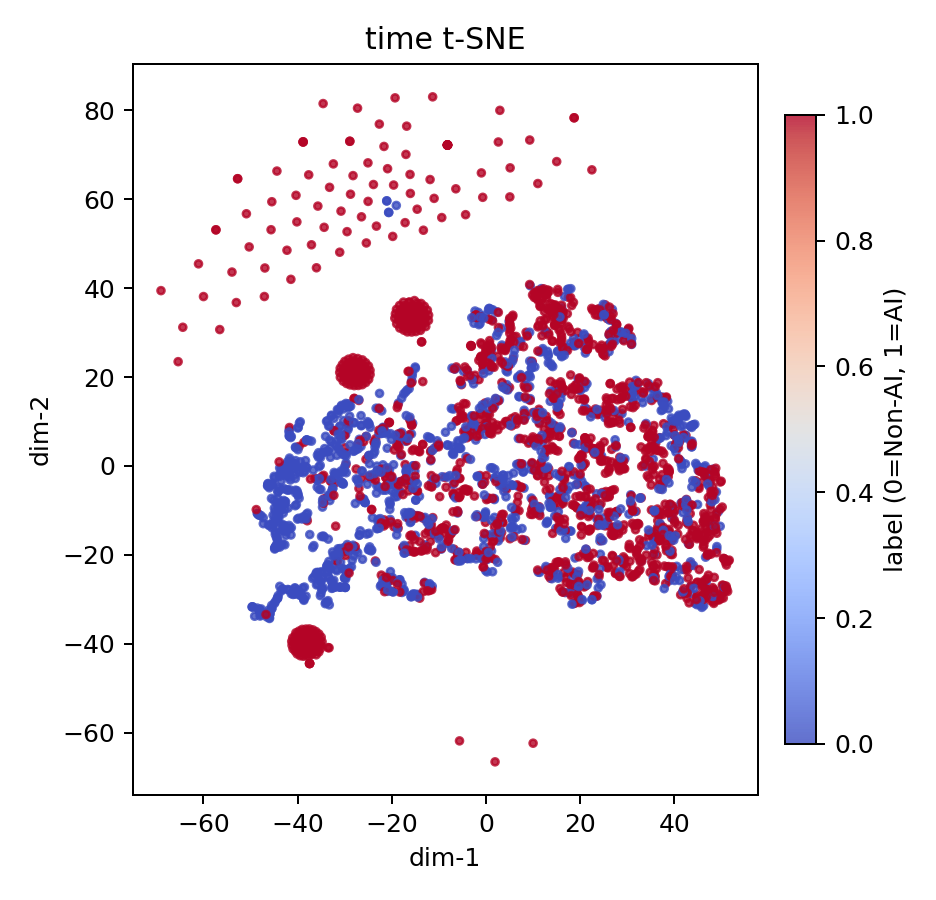
\includegraphics[width=.4\linewidth]{images_in_paper/embed_time_tsne.png}
%   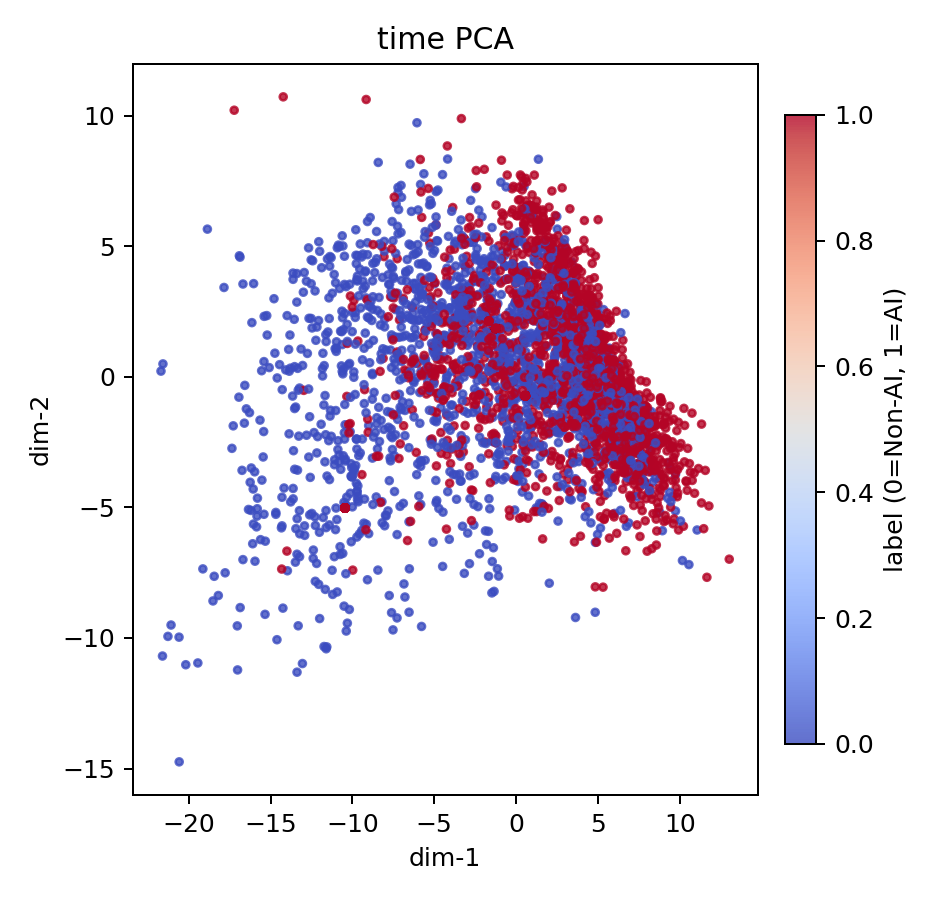
\includegraphics[width=.4\linewidth]{images_in_paper/embed_time_pca.png}
%   \caption{时域分支嵌入:t-SNE(左)与 PCA(右)。}
%   \label{fig:time_tsne}
%   \label{fig:time_pca}
% \end{figure}
%
% 相对地,formant 分支(图~\ref{fig:formant_tsne})总体上红蓝高度交织,仅在若干局部“岛状”区域聚集,
% 表明\emph{整体}频谱包络并不足以稳定区分全部 AI 样式,但对特定风格(如固定声道/共振峰模板)的 AI 样本存在\emph{局部}可分性。
%
% \begin{figure}[H]
%   \centering
%   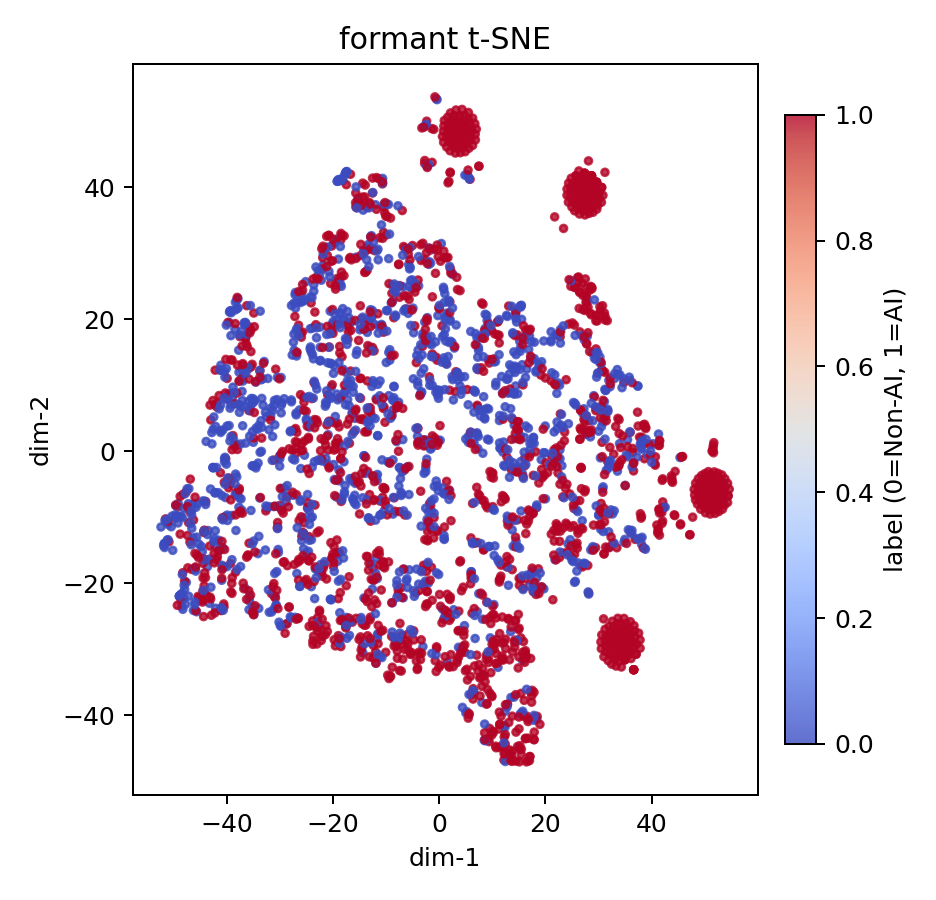
\includegraphics[width=.4\linewidth]{images_in_paper/embed_formant_tsne.png}
%   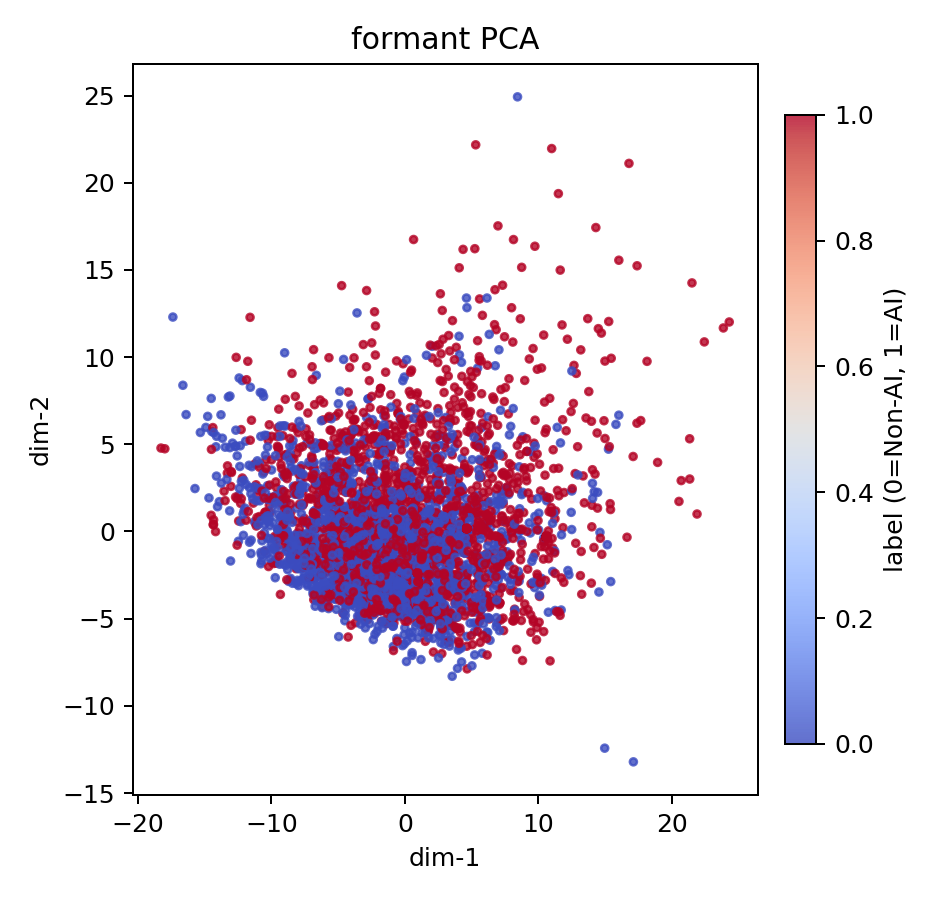
\includegraphics[width=.4\linewidth]{images_in_paper/embed_formant_pca.png}
%   \caption{formant 分支嵌入:t-SNE(左)与 PCA(右)。}
%   \label{fig:formant_tsne}
%   \label{fig:formant_pca}
% \end{figure}
%
% \paragraph{(2)量化分析:有针对性的微扰能显著改变判别。}
% 我们对相同音源施加多类微扰并记录主分类概率($\mathrm{prob\_main}$)变化。
% 结果表明,\emph{时域动态扰动}(\texttt{timeDyn\_strong/medium/\ldots})与
% \emph{类共振峰扰动}(\texttt{formantish\_strong/medium/\ldots})可将判别概率稳定压低
% (例如 \texttt{timeDyn\_strong} $\approx 0.24$,\texttt{formantish\_strong} $\approx 0.30$),
% 显著低于原始片段;而单纯的高频窄带 EQ 微调(如 $15$\,kHz、$\pm(0.8\!\sim\!1.8)$\,dB)影响较弱。
% 结合探针头输出可见,时域与 formant 分支单独判断时的 AI 概率降幅最大,表明模型决策高度依赖
% \textbf{时域包络/动态}与\textbf{人声共振峰布局}两类特征;一旦这些特征被微调,决策边界即向“非 AI”区域偏移。
%
% 为了初步分析各个分支对最终决策的决策方向的影响,我们构造了如下两个指标来进行量化分析:
% \begin{itemize}
%   \item \textbf{logit}:
%   模型主分类器在融合所有分支嵌入后的线性层输出(未经过 Sigmoid)。
%   logit 值的正负反映了模型决策的方向(正值偏向 AI,负值偏向非 AI),绝对值大小反映了决策的置信度。
%   在分析中,logit 可作为样本被判定为 AI 或非 AI 的“力度”指标,用于衡量扰动前后决策信号的变化。
%
%   \item \textbf{contrib}:
%   按分支拆分最终线性层权重,对该分支嵌入向量与权重做点积,得到该分支对 logit 的加和贡献。
%   若无法直接分块,可用 Grad$\times$Input 在分支拼接点近似计算。
%   贡献值为正表示该分支推动决策向 AI 方向,为负则推动向非 AI 方向。
%   通过统计 contrib 值的分布与类别差异,可以识别在整体判决中起主导作用的分支,并结合扰动实验分析其易受攻击性。
% \end{itemize}
%
% 图~\ref{fig:contrib_means} 展示了不同分支在 AI 与非 AI 样本上的平均贡献值及标准误差。
% 可以看到,\texttt{spec} 分支在两类样本中均呈显著正贡献(推高 AI 判别概率),
% \texttt{time} 分支则整体呈负贡献(抑制 AI 判别),且幅度较大;
% \texttt{prosody}、\texttt{formant} 与 \texttt{hjorth} 分支的贡献幅度较小,
% 说明在多数样本中,它们对最终判别的直接推动作用有限。
%
% \begin{figure}[H]
%   \centering
%   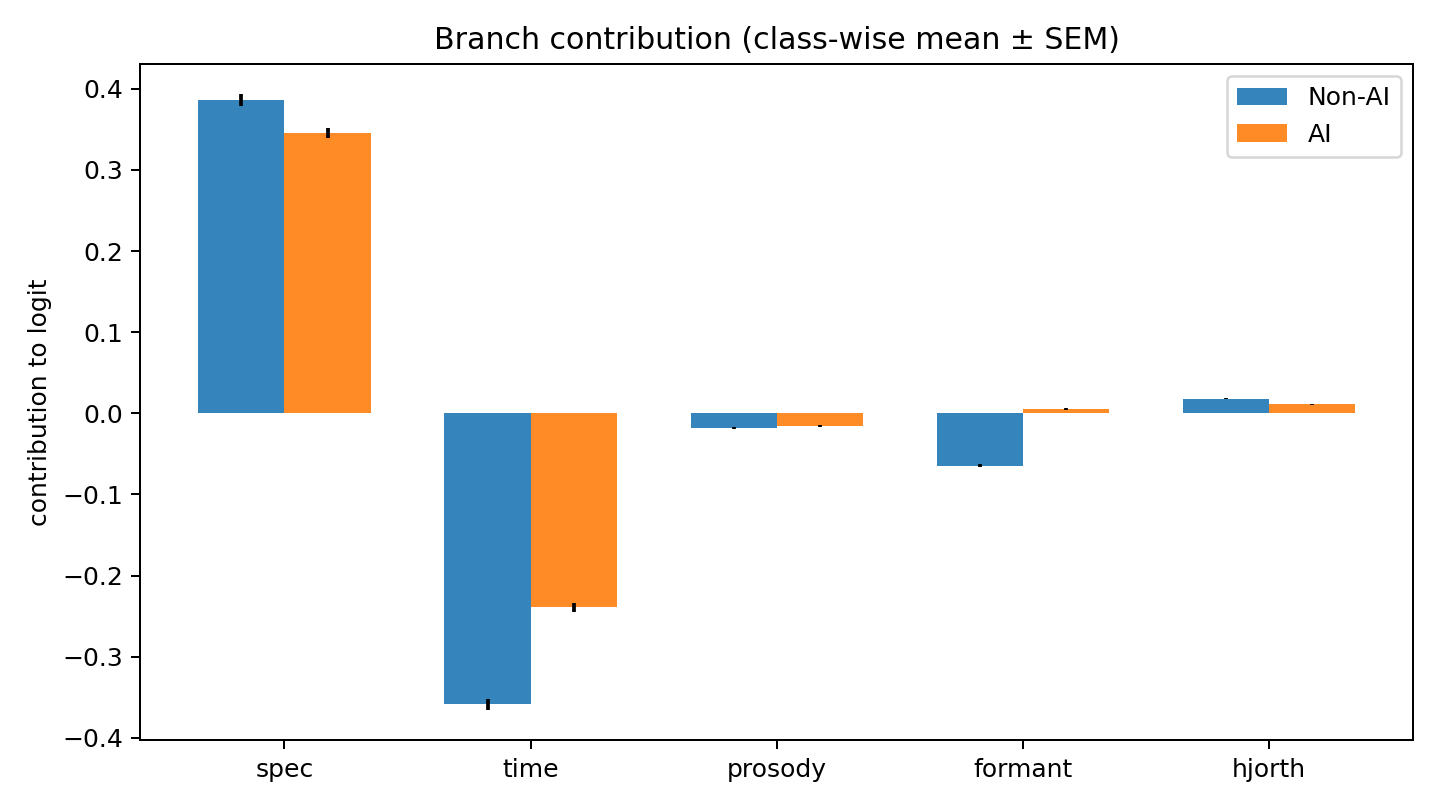
\includegraphics[width=.75\linewidth]{images_in_paper/contrib_means_by_class.png}
%   \caption{不同分支在 AI 与非 AI 样本上的平均 logit 贡献(均值 $\pm$ SEM)。}
%   \label{fig:contrib_means}
% \end{figure}
%
% 为了考察分支贡献的相关性,我们计算了样本层面的皮尔逊相关系数矩阵(图~\ref{fig:contrib_corr})。
% 结果显示,\texttt{spec} 与 \texttt{time} 分支呈显著负相关,
% 表明它们在多数样本的决策中存在一定的“对冲”关系——当一个分支强烈推动向 AI 方向时,另一个分支往往抑制该判别。
% 此外,\texttt{prosody} 与 \texttt{time}、\texttt{formant} 的正相关,说明这些分支在部分样本中可能协同作用。
%
% \begin{figure}[H]
%   \centering
%   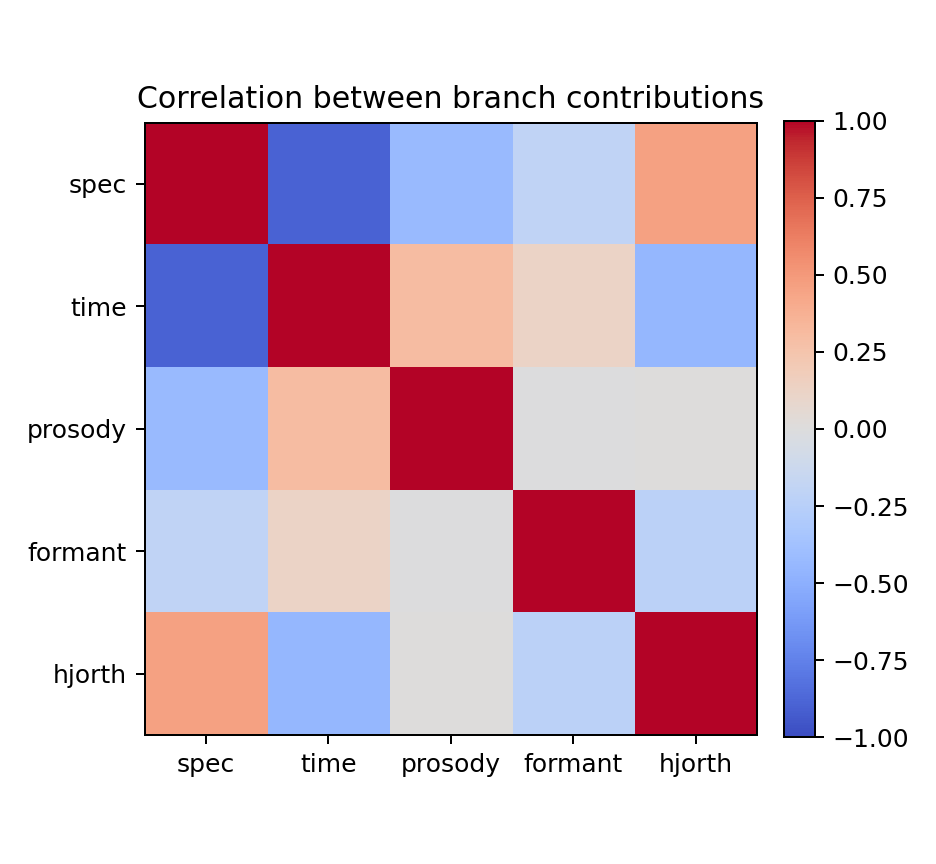
\includegraphics[width=.5\linewidth]{images_in_paper/contrib_correlation.png}
%   \caption{各分支 logit 贡献的相关性矩阵(皮尔逊相关系数)。}
%   \label{fig:contrib_corr}
% \end{figure}
%
% 图~\ref{fig:contrib_violin} 给出了所有样本的分支贡献分布。
% 可以看出,\texttt{time} 分支的贡献分布跨度最大,从强负到强正均有覆盖,说明它在部分样本中具有极高的判别权重,而在另一些样本中几乎不参与判别;
% \texttt{spec} 分支则分布相对集中且整体偏正,体现了其在多数样本中稳定推高 AI 判别的趋势;
% \texttt{formant} 分支分布较分散,但极端值较多,可能在某些特定声学风格下起关键作用。
%
% \begin{figure}[H]
%   \centering
%   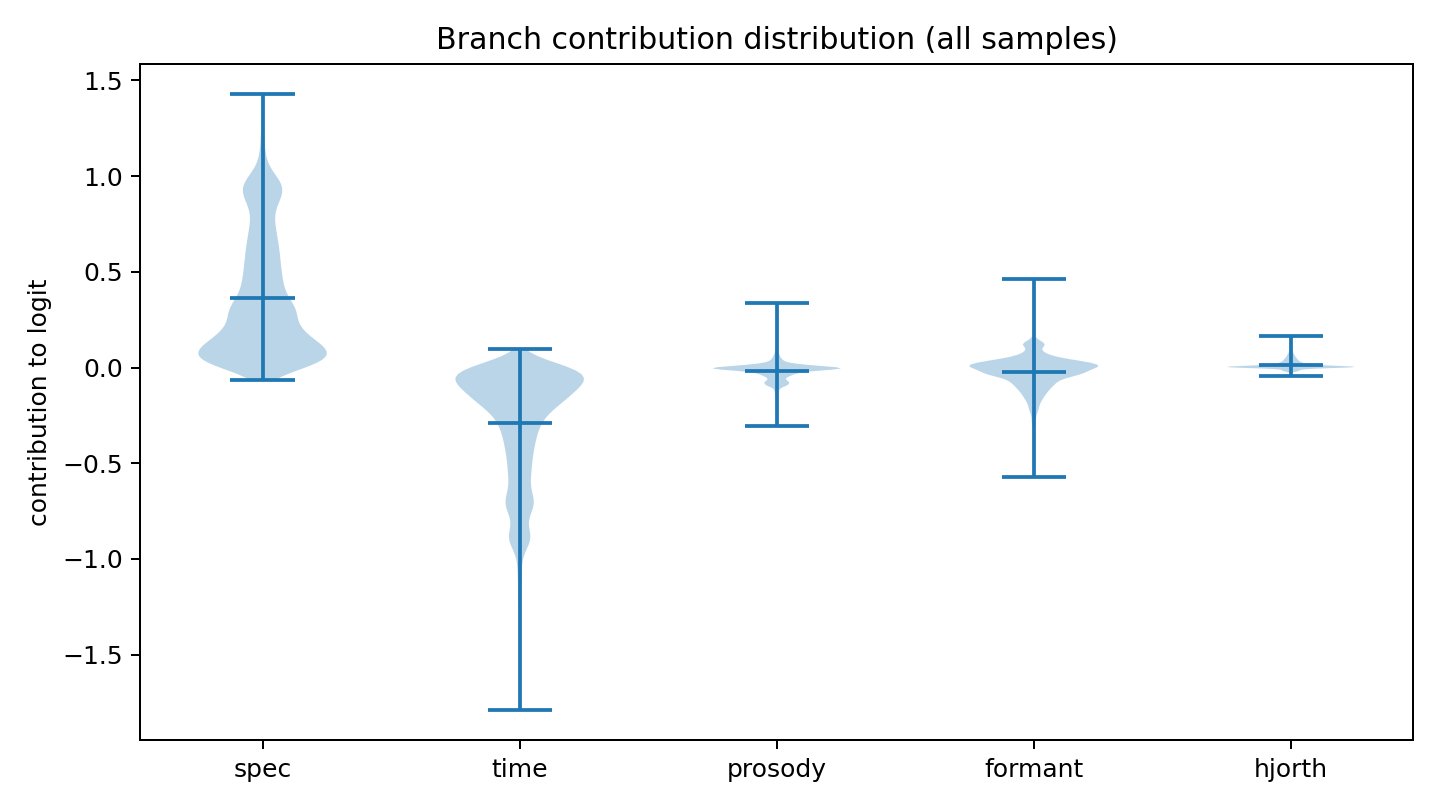
\includegraphics[width=.75\linewidth]{images_in_paper/contrib_violin_all.png}
%   \caption{各分支 logit 贡献的分布(所有样本)。}
%   \label{fig:contrib_violin}
% \end{figure}
%
% 我们为每个分支计算了如下指标,表征其决策能力,分析最终决策对各个分支的依赖性:
%
% \begin{itemize}
%   \item \textbf{AUC(Area Under the ROC Curve)}:
%   表示在所有可能的分类阈值下,模型正确区分正负样本的概率,由此绘制出图~\ref{fig:roc}。
%   ROC曲线数据点越集中在左上角,则特定阈值下召回率与误报率之比越高,AUC 值越接近 1,说明该分支嵌入在全范围阈值下的判别能力越强;
%   AUC = 0.5 表示无判别能力,相当于随机猜测。
%
%   \item \textbf{ACC(Accuracy)}:
%   表示在固定分类阈值(本文取 0.5)下,分支嵌入在验证集上的分类准确率。
%   ACC 关注的是单一阈值下的硬判别性能,反映该分支在常规决策条件下的直接预测效果。
%
%   \item \textbf{Fisher\_mean}:
%   衡量类间分离度与类内紧凑度的比值。其定义为:
%   \[
%   \text{Fisher Ratio} = \frac{\sum_d (\mu_d^{+} - \mu_d^{-})^2}{\sum_d (\sigma_d^{+2} + \sigma_d^{-2})}
%   \]
%   其中 $\mu_d^{+}$ 和 $\mu_d^{-}$ 分别为第 $d$ 维在正、负样本上的均值,
%   $\sigma_d^{+2}$ 和 $\sigma_d^{-2}$ 为对应方差。
%   Fisher 比率越大,说明该分支的嵌入向量在不同类别间分布差异更明显,且类内方差更小,有利于判别。
%
% \end{itemize}
%
% 这种扰动敏感性与分支的单独判别能力高度一致:
% 定量评估显示,时域分支在 5 折交叉验证下的 AUC 达到 $0.8251\!\pm\!0.0076$,
% ACC 为 $0.7627\!\pm\!0.0025$,Fisher 比率 $0.1324$;
% formant 分支的 AUC 为 $0.8161\!\pm\!0.0077$,ACC 为 $0.7413\!\pm\!0.0101$,
% Fisher 比率 $0.0912$。
% 两者均显著高于 prosody(AUC $0.7191$,Fisher $0.0071$)与 hjorth(AUC $0.6963$,Fisher $0.0054$)等弱分支,
% 说明模型在融合决策时,确实更依赖时域包络/动态与人声共振峰布局等特征;
% 当这两类特征被结构性微调时,主分类概率便会大幅偏向“非 AI”区域。
%
% \begin{figure}[H]
%   \centering
%   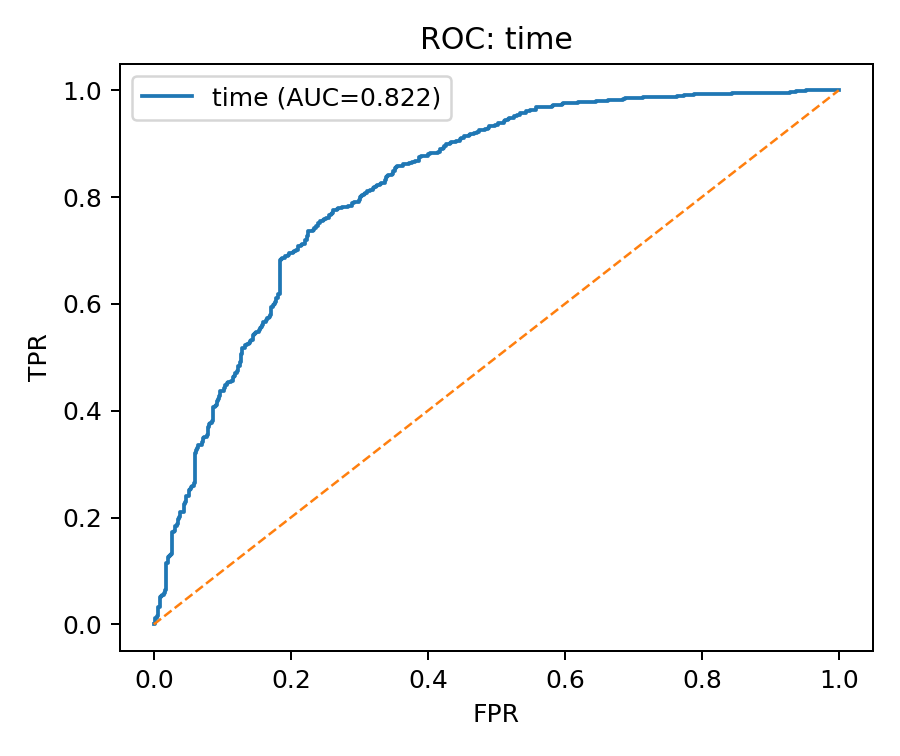
\includegraphics[width=.45\linewidth]{images_in_paper/roc_time.png}
%   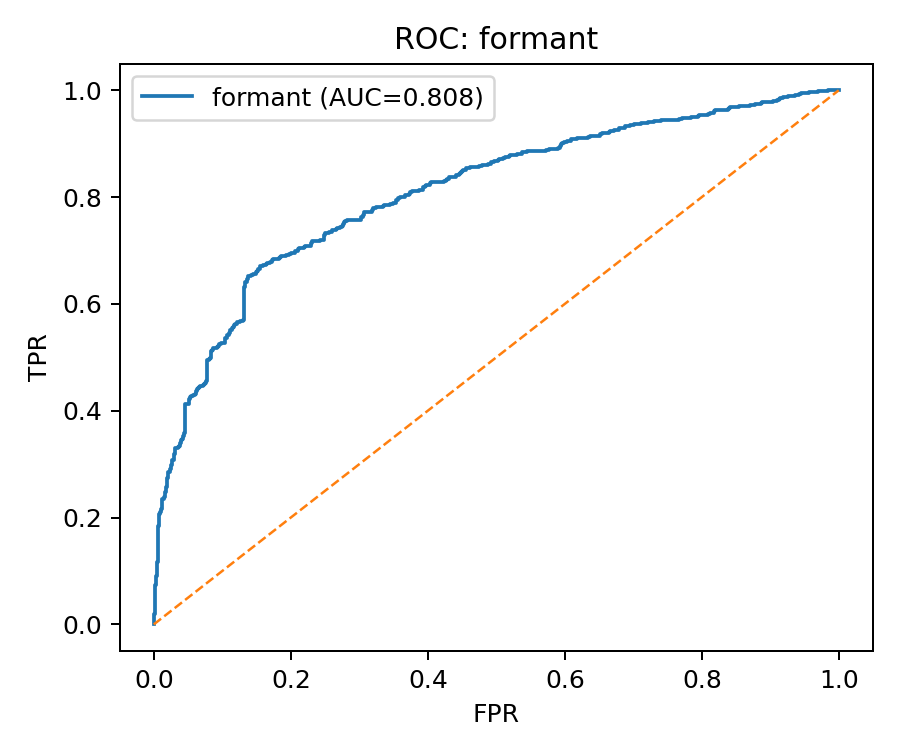
\includegraphics[width=.45\linewidth]{images_in_paper/roc_formant.png}
%   \caption{时域分支与 formant 分支 ROC 曲线。}
%   \label{fig:roc}
% \end{figure}
%
% \begin{figure}[H]
%   \centering
%   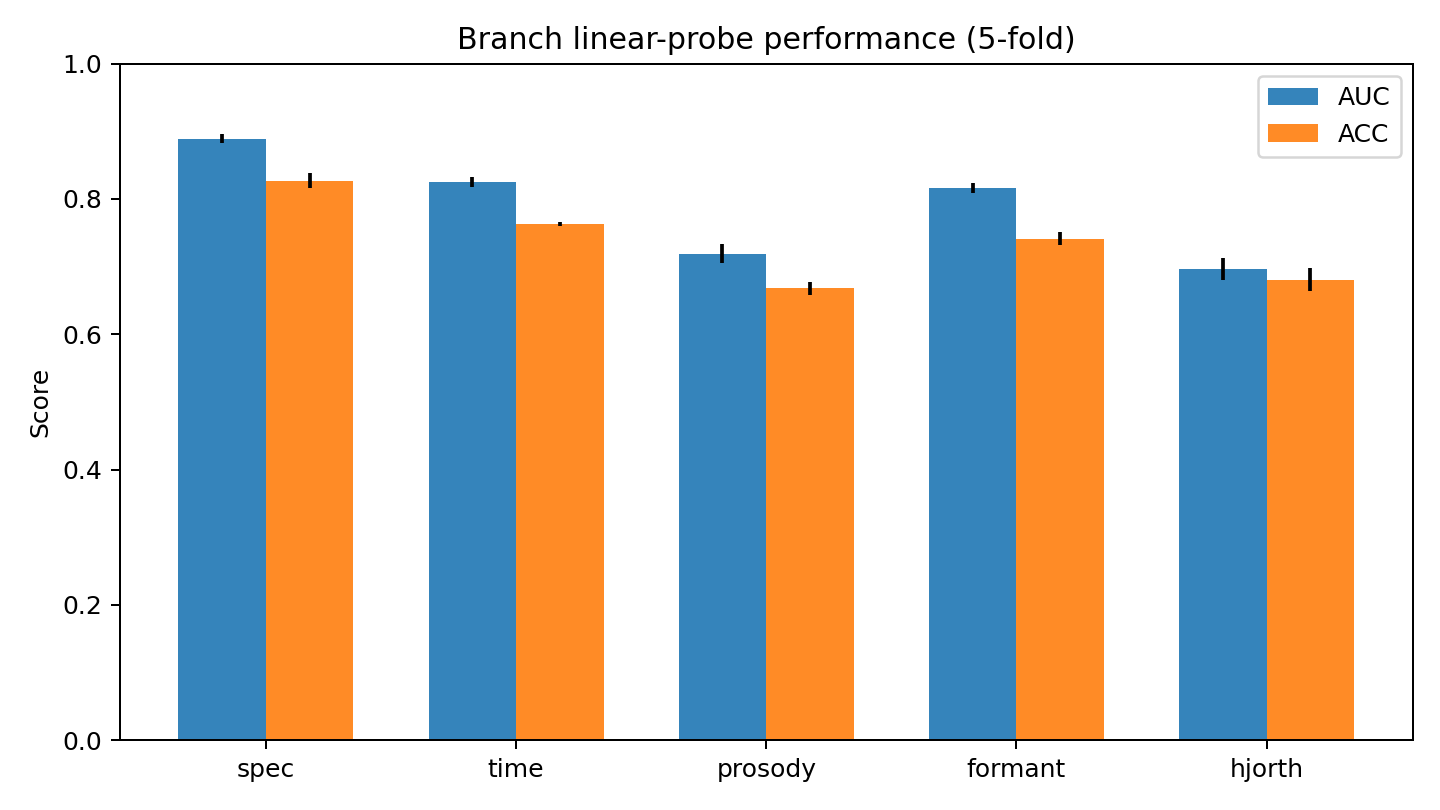
\includegraphics[width=.32\linewidth]{images_in_paper/branch_metrics_auc_acc.png}
%   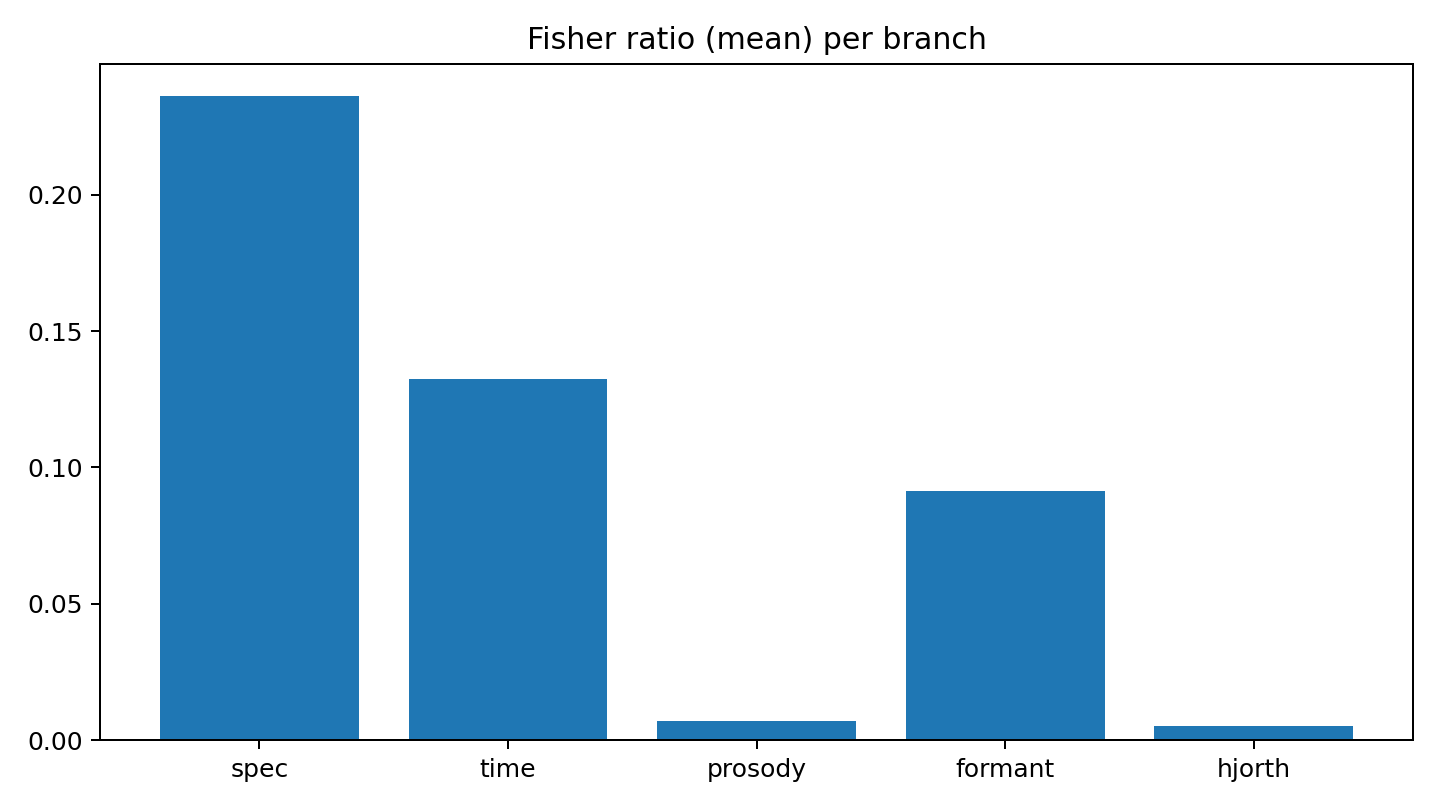
\includegraphics[width=.32\linewidth]{images_in_paper/branch_fisher.png}
%   \caption{分支可分性定量指标:AUC/ACC(中)、Fisher 比率(右)。}
%   \label{fig:branch_silhouette}
%   \label{fig:branch_aucacc}
%   \label{fig:branch_fisher}
% \end{figure}
%
%
% \paragraph{(3)偏差与失败模式。}
% 在排序表中,自然环境纹理(如雨声、林声、城市公园环境)也获得较低的 AI 概率,提示模型对\emph{非乐音/非稳态}素材存在天然“真值”偏好,
% 可能源于训练集分布差异(音乐性与稳态谐波成分占比更高)。
% 这类偏差意味着:通过\emph{轻度压缩+全通相位}改变瞬态,以及\emph{小幅峰值 EQ} 微移 formant,即可在不破坏主观听感的前提下,提高“过检”概率。
%
% \subsubsection{改进方向}
% 综合嵌入结构与扰动响应,我们将特征归因排序为:\textbf{时域动态(首要)} $>$ \textbf{频谱包络/共振峰(次要)} $>$ \textbf{高频细窄带均衡(较弱)}。
% 为缓解脆弱性,未来可以考虑在训练中加入:(i)动态压缩、全通相位、微小时间伸缩的强数据增强;(ii)formant 随机漂移/声道随机化;
% (iii)在多分支架构上引入一致性正则或分支 dropout,以降低单一分支的主导性,并对自然环境纹理补充“反例”样本以纠正数据偏差。
%
% \section{模型优缺点与推广}
%
% \begin{frame}[fragile,allowframebreaks]{模型优缺点与推广}
% \small
% \paragraph{模型优点} 
% 本文提出的多分支 CNN 检测模型能够同时处理时域、频域、音高与音质等多种声学特征,结构上实现了多源信息的并行提取与融合,充分利用了不同特征维度之间的互补性。实验结果表明,该模型在常规测试集上取得了较高的分类准确率(验证集稳定在 89\%--90\%),且在多数轻中度扰动条件下保持了良好的检测性能;在较强扰动下,全连阶层输出的AI判别概率会有明显扰动,但是,综合五个分支探针头的概率计算出的AI痕迹评分(式~\ref{eq:ai_score}),在强扰动下仍然坚挺;由此可见模型具备一定的泛化能力与鲁棒性。此外,模型规模相对轻量,计算开销低,易于在多平台部署,并可支持实时检测需求。
%
% \paragraph{模型不足} 
% 尽管整体性能优良,但鲁棒性分析发现模型在高频噪声注入(highFreqInject)与环境噪声混入(ambientNoise)等特定扰动下的检测概率显著下降,表明在面对宽带噪声和高频干扰时的特征表达仍存在脆弱性。此外,当前特征融合层为固定权重,未能根据输入特征的质量动态调整各分支贡献,这在某些特征受扰较大的情况下可能限制了模型的自适应能力。训练数据主要集中于有限风格与生成引擎,对极端风格、全新算法生成的音乐仍可能存在适配不足。
%
% \paragraph{模型推广} 
% 该多分支 CNN 框架具备良好的可扩展性,可根据不同检测任务灵活替换或新增特征分支。例如,在语音深度伪造检测中,可增加语音特有的相位一致性特征分支;在环境音场景识别中,可引入空间声学特征分支。模型也可与自编码器异常检测方法结合,用自监督方式预训练分支特征提取器,再进行有监督分类,从而提升在低资源或开放域场景下的表现。进一步地,可将该方法与传统机器学习特征融合(如 XGBoost、SVM)进行混合,形成多模态、多尺度的综合检测框架,推广到更多 AI 音频内容安全相关领域。
%
% \appendix
% \end{frame}
\begin{frame}[standout]
  谢谢大家!
\end{frame}
\end{document}
